\documentclass[conference,a4paper]{ieeetran}

\usepackage[latin1]{inputenc}
\usepackage{subeqnarray}
\usepackage{amsfonts}
\usepackage{amsmath}
\usepackage{amssymb}
\usepackage{graphicx}
\usepackage{color}
\parskip 1mm
\arraycolsep 0.5mm
\newtheorem{theorem}{Theorem}
\newcommand{\sign}{\mathrm{sign}}
\newcommand{\sat}{\mathrm{sat}}

\title{International Conference on Image Processing Theory, Tools and Applications}

\author{\authorblockN{Author\authorrefmark{1}, Author\authorrefmark{1} and Author\authorrefmark{2} }
\authorblockA{\authorrefmark{1} Affiliation 1\\
e-mail: author-1@ieee.org, author-2@ieee.org}
\authorblockA{\authorrefmark{2} Affiliation 2\\
e-mail: author-3@ieee.org}}

\begin{document}
\maketitle
\begin{abstract}
\texttt{ieeetran} is a modified version of the \texttt{IEEEtran}
class. This document describes how to use \texttt{ieeetran} class
with \LaTeX{} to produce high quality typeset papers that are
suitable for submission to the International Conference on Image
Processing Theory, Tools and Applications. Authors are kindly
requested to follow the instructions found in this document.
\end{abstract}

\begin{keywords}
    Image processing theory, Image processing tools, Image processing applications, Template, Typesetting.
\end{keywords}

\section{Introduction}
The international conference on Image Processing Theory, Tools and
Applications aims at gathering challenging international
researchers, innovators, educators, and practitioners in image
processing theory and tools, for attending extensive educational
high level materials, sharing their achievements, exchanging their
experiences and discussing future orientations.

By using the \texttt{ieeetran} class file, a computer running \LaTeX{}, and a basic
understanding of the \LaTeX{} language, an author can produce professional quality
typeset research papers very quickly, inexpensively, and with minimal effort. The purpose
of this document is to serve as a user guide of \texttt{ieeetran} \LaTeX{} class.

It is assumed that the reader has at least a basic working knowledge of \LaTeX{}. Those so lacking
are strongly encouraged to read some of the excellent literature on the subject. We refer the
reader to the following sites: \texttt{\textcolor[rgb]{0.00,0.00,1.00}{http://tex.loria.fr}} and
\texttt{\textcolor[rgb]{0.00,0.00,1.00}{http://www.miktex.org}}.

Please note that your paper should normally be limited to six pages.


\section{Headings}
This part of the document containing its title, author names and affiliations.

\subsection{Paper title}
The paper title is inserted as follows:
\begin{verbatim}
\title{Title of the paper}
\end{verbatim}
Line breaks (\verb"\\") may be used to equalize the length of the title lines.

\subsection{Author names and affiliations}
Author names and associated information are declared as follows: {\small
\begin{verbatim}
\author{\authorblockN{
 Michael Shell\authorrefmark{1},
 Homer Simpson\authorrefmark{2},
 James Kirk\authorrefmark{3},
 Montgomery Scott\authorrefmark{3}
 and Eld on Tyrell\authorrefmark{4}}
\authorblockA{\authorrefmark{1}
School of Electrical a
nd Computer Engineering\\
Georgia Institute of Technology,
Atlanta, Georgia 30
332--0250\\
email: mshell@ece.gatech.edu}
\authorblockA{\authorrefmark{2}
Twentieth Century Fox, Springfield, USA\\
email: homer@thesimpsons.com}
\authorblockA{\authorrefmark{3}
Starfleet Academy, Sa n Francisco,
California 96678-2391}
\authorblockA{\authorrefmark{4}
Tyrell Inc., 123 Replicant Street,
 Los Angeles, California 90210--4321}}
\end{verbatim}}
\section{Abstract and keywords}
The abstract is generally the first part of a paper. The abstract text is placed within the
abstract environment:
\begin{verbatim}
\begin{abstract}
This paper deals with ...
\end{abstract}
\end{verbatim}
The IPTA papers should also include a list of (4 to 6) key words which can be declared
within the \texttt{keywords} environment:
\begin{verbatim}
\begin{keywords}
    Image processing theory, Image
    processing tools, Image processing
    applications, Template, Typesetting.
\end{keywords}
\end{verbatim}

\section{Sections}
Sections and their headings are declared in the usual \LaTeX{} fashion via \verb"\section{}",
\verb"\subsection{}", \verb"\subsubsection{}", and \verb"\paragraph{}". The numbering for these
sections is in arabic numerals except for \verb"\paragraph{}" which is not numbered because,
generally, papers should not have such a deep section nesting depth.

\section{Mathematical formulas}
Mathematical formulas are created using the standard \LaTeX{} environments such as:
\begin{verbatim}
\begin{equation}
    \label{MPKeq1}
    x^2+2x+5=0
\end{equation}
\end{verbatim}
which yields:
\begin{equation}
    \label{MPKeq1}
    x^2+2x+5=0
\end{equation}

For long equations that do not fit to the column width one can use the \verb"\split"
environment{\footnotesize
\begin{verbatim}
\begin{equation}
 \label{MPKeq2}
 \begin{split}
 y(t) = &\left\{\frac{\tau^n \sin n\pi}{\pi}
 \int_0^\infty \frac{x^n e^{-xt}dx}
 {1+2(\tau x)^n\cos n\pi+(\tau x)^{2n}}\right\}u(t)\\
 &-\left\{\frac{2}{n}\tau^{-1}e^{t\tau^{-1}
 \cos\frac{\pi}{n}}\cos\left(t\tau^{-1}
 \sin\frac{\pi}{n}+\frac{\pi}{n}\right)\right\}u(t).
 \end{split}
\end{equation}
\end{verbatim}}
which yields:
\begin{equation}
    \label{MPKeq2}
    \begin{split}
    y(t) = &\left\{ {\frac{{\tau ^n \sin n\pi }}{\pi
    }\int_0^\infty  {\frac{{x^n e^{ - xt} dx}}{{1 + 2\left( {\tau x} \right)^n \cos n\pi  +
    \left( {\tau x} \right)^{2n} }}} } \right\}u\left( t \right) \\
    &- \left\{ {\frac{2}{n}\tau ^{ - 1} e^{t\tau ^{ - 1} \cos \frac{\pi }{n}} \cos \left( {t\tau ^{ -
    1} \sin \frac{\pi }{n} + \frac{\pi }{n}} \right)} \right\}u\left( t \right).
    \end{split}
\end{equation}

\section{Figures}
Figures are handled in the standard \LaTeX{} manner. For example:
\begin{verbatim}
\begin{figure}[!ht]
\centering
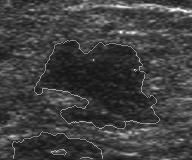
\includegraphics[width=7cm]{coeur3.png}
\caption{Inverted pendulum.}
\label{MPKfig1}
\end{figure}
\end{verbatim}
The \verb"\includegraphics" command is the modern, preferred, way of including images and provides
a flexible interface that makes it easy to scale graphics to size. To use it, the  \verb"graphicx"
package must first be loaded:
\begin{verbatim}
\usepackage{graphicx}
\end{verbatim}
Note that: (1) figures should be centered via the \LaTeX{} \verb"\centering" command. This is a
better approach than using the \verb"center" environment which adds unwanted vertical spacing; (2)
the caption follows the graphic; and (3) any labels must be declared after (or within) the caption
command. When referencing figure numbers in the main text (via \verb"\ref{}"), authors should use
the abbreviation ``Fig." rather than ``Figure" except when starting the sentence. For example:

\begin{figure}[!ht]
    \centering
    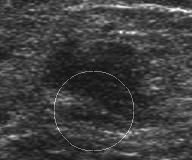
\includegraphics[width=4cm]{coeur0.PNG}
    \caption{Initialization.}
    \label{MPKfig1}
\end{figure}
Figure \ref{MPKfig1} shows the initialization step. Image
segmentation is showed in Fig. \ref{segmentation}.

\begin{figure}[htpb]
    \begin{center}
    \resizebox{4cm}{!}{     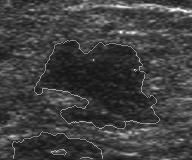
\includegraphics{coeur3.PNG}}
\end{center}
\caption{Image segmentation: Convergence towards final contours.}
\label{segmentation}
\end{figure}

The above figure is created using the freeware \verb"Ipe6.0 preview23" available on the following
site \verb"http://ipe.compgeom.org/".

Encapsulated postscript (\texttt{.eps}) figures can be generated from MATLAB by typing the
following in the command window: \\ \texttt{print filename.eps -depsc}.

\section{Tables}
Tables are defined in the same manner as figures except that captions should appear above
the tables. When referencing table numbers in the main text no abbreviation is used. Next
we can see an example of a table:{\small
\begin{verbatim}
\begin{table}[!ht]
\centering
\caption{Accuracy recognition.}
    \begin{tabular}{|l|c|c|c|}
    \hline
     & \multicolumn{3}{c|}
     {Classification algorithms}\\
    \cline{2-4}
     & SVM & RBF & MLP
     \hline
     Precision & 98.79\%& 83.71\%& 88.11\%\\
     Recall & 93.33\%& 81.6\%& 85.33\%\\
     \hline
    \end{tabular}
\end{table}
\end{verbatim}}
produces
\begin{table}[!ht]
    \centering
    \caption{Accuracy recognition.}
    \begin{tabular}{|l|c|c|c|}
        \hline
         & \multicolumn{3}{c|}{Classification algorithms}\\
         \cline{2-4}
         & SVM & RBF & MLP\\
        \hline
        Precision & 98.79\%& 83.71\%& 88.11\%\\
        Recall & 93.33\%& 81.6\%& 85.33\%\\
        \hline
    \end{tabular}
    \label{MPKtab1}
\end{table}



\section{Citation}
Citations are made using the standard \LaTeX{} command \verb"\cite{}", this will produce a number
inside square brackets. Multiple citations are included within one \verb"\cite{}" command separated
with commas. \emph{e.g.}

Segmentation systems are studied in \cite{Pattern recognition,phdthesis}.\\
(\verb"\cite{Pattern recognition,phdthesis}")

For more details on restoration of images corrupted by impulse
noise, the reader is referred to \cite{IEEE Transactions}.
(\verb"\cite{IEEE Transactions}")

\section{References}
References are declared at the end of the article within the \texttt{thebibliography} environment.
\begin{verbatim}
\begin{thebibliography}{1}
\bibitem{}...

\bibitem{}...

\end{thebibliography}
\end{verbatim}

Journal articles are declared as follows, where the volume number is a necessary entry
and the number of the issue is optional and put in parenthesis:{\small
\begin{verbatim}
\begin{thebibliography}{1}
\bibitem{Pattern recognition}
H. L. Premaratne and J. Bigun.
\newblock A segmentation-free
approach to recognise printed
Sinhala script using linear
symmetry.
\newblock {\em Pattern Recognition},
37(10): 2081--2089, 2004.

\bibitem{IEEE Transactions}
M. E. Yuksel.
\newblock A hybrid neuro-fuzzy filter
for edge preserving restoration
of images corrupted by impulse noise.
\newblock {\em IEEE Trans. on Image
Processing}, 15(4): 928--936, 2006.
\end{thebibliography}
\end{verbatim}}

PhD theses and conference articles are declared as follows:{\small
\begin{verbatim}
\begin{thebibliography}{1}
\bibitem{phdthesis}
C. Tauber.
\newblock {\em Filtrage anisotrope
robuste et segmentation par B-spline snake
: application aux images �chographiques}.
\newblock PhD thesis, Toulouse National
Polytechnic Institute, Toulouse-France, 2005.

\bibitem{Conference}
P. Ziaie, T. Muller and A. Knoll.
\newblock A Novel Approach to Hand-Gesture
Recognition in a Human-Robot Dialog System.
\newblock In {\em First Int. Workshops on
Image Processing Theory, Tools and
Applications (IPTA'08)},
proceedings, Sousse-Tunisia,  November 2008.
\end{thebibliography}
\end{verbatim}}

\section{Appendix}
The appendix is declared using the command
 \verb"\appendix[title of appendix]", if only one appendix is to be included. If more than one appendix will be
included then we use the command \verb"\appendices" and then we use
 \verb"\section{title of appendix}" Inside the appendix subsections are not allowed.
\appendices
\section{theorem 1}
\begin{theorem}
Suppose $c \geq 0,~~r(.)$ and $k(.)$ are nonnegative valued continuous functions, and suppose
\begin{equation}
    \label{app1}
    r(t) \leq c+ \int _{0}^{t} k(\tau)r(\tau)d\tau,~~~~\forall t \in [0,T]
\end{equation}
Then
\begin{equation}
    \label{app2} r(t) \leq c~ \exp \left[ \int _{0}^{t} k(\tau)d\tau \right],~~~~\forall t \in [0,T]
\end{equation}
\end{theorem}
\section{Lyapunov equation} The equations in the appendix are numbered with the corresponding appendix
letter.
\begin{equation}
    A^TP+PA=-Q
\end{equation}

\section*{Acknowledgment}
 The author would like to thank all those who have helped in the realization of this
document.

Acknowledgment is added as an unnumbered section using the standard \LaTeX{} command
\verb"\section*{Acknowledgment}".

\begin{thebibliography}{1}

\bibitem{Pattern recognition}
H. L. Premaratne and J. Bigun.
\newblock A segmentation-free approach to recognise printed Sinhala script using linear symmetry.
\newblock {\em Pattern Recognition}, 37(10): 2081--2089, 2004.


\bibitem{phdthesis}
C. Tauber.
\newblock {\em Filtrage anisotrope robuste et segmentation par B-spline snake
: application aux images �chographiques}.
\newblock PhD thesis, Toulouse National Polytechnic Institute, Toulouse-France, 2005.


\bibitem{IEEE Transactions}
M. E. Yuksel.
\newblock A hybrid neuro-fuzzy filter for edge preserving restoration
of images corrupted by impulse noise.
\newblock {\em IEEE Trans. on Image Processing}, 15(4): 928--936, 2006.


\bibitem{Conference}
P. Ziaie, T. Muller and A. Knoll.
\newblock A Novel Approach to Hand-Gesture Recognition in a Human-Robot Dialog System.
\newblock In {\em First Int. Workshops on Image Processing Theory, Tools and Applications (IPTA'08)},
proceedings, Sousse-Tunisia,  November 2008.


\end{thebibliography}

\end{document}
